\section{Methods}

Liquid-fueled system modeling with contemporary reactor physics codes is 
difficult because most of these codes were developed for analyzing solid-fueled 
reactors. In fact, world-wide commercial reactors fleet today is represented by 
systems with solid fuel. Liquid-fueled systems ability to continuously remove 
fission products and add fissile and/or fertile elements is the main challenge 
for depletion simulations. SaltProc takes into account online separations and 
feeds using SERPENT 2 continuous-energy Monte Carlo neutron transport and 
depletion code.

\subsection{Molten Salt Breeder Reactor design and model description}
The \gls{MSBR} vessel has a diameter of 680 cm and a height of 610 cm. It 
contains a molten fluoride fuel-salt mixture that generates heat in the active 
core region and transports that heat to the primary heat exchanger by way of 
the primary salt pump. In the active core region, the salt flows through 
channels in moderating and reflecting graphite blocks. Salt at about 
565$^{\circ}$C enters the central manifold at the bottom via four 
40.64-cm-diameter nozzles and flows upward through channels in the lower plenum 
graphite. The fuel salt exits at the top at about 704$^{\circ}$C through four 
equally spaced nozzles which connect to the salt-suction pipes leading to 
primary circulation pumps. The fuel salt drain lines connect to the bottom of 
the reactor vessel inlet manifold.

Figure~\ref{fig:serpent_plan_view} demonstrate the configuration of the 
\gls{MSBR} vessel, core configuration, ``fission" (zone I) and ``breeding" 
(zone II) regions inside the vessel. The core has two radial zones bounded by a 
solid cylindrical graphite reflector and the vessel wall. The central zone, 
zone I, in which 13\% of the volume is fuel salt and 87\% graphite. Zone I 
composed of 1,320 graphite cells, 2 graphite control rods, and 2 
safety\footnote{ These rods needed for emergency shutdown only.} rods. The 
under-moderated zone, zone II, with 37\% fuel salt, and radial reflector, 
surrounds the zone I core region and serves to diminish neutron leakage. Zones 
I and II are surrounded radially and axially by fuel salt 
(figure~\ref{fig:serpent_zoneII}). This space for fuel is necessary for 
injection and flow of molten salt.

Since reactor graphite experiences significant dimensional changes due to 
neutron irradiation, the reactor core was designed for periodic replacement. 
Based on the irradiation experimental data from \gls{MSRE}, core graphite 
lifetime is about 4 years and reflector graphite lifetime is 30 years 
\cite{robertson_conceptual_1971}.

\begin{figure}[hbp!] % replace 't' with 'b' to \centering
  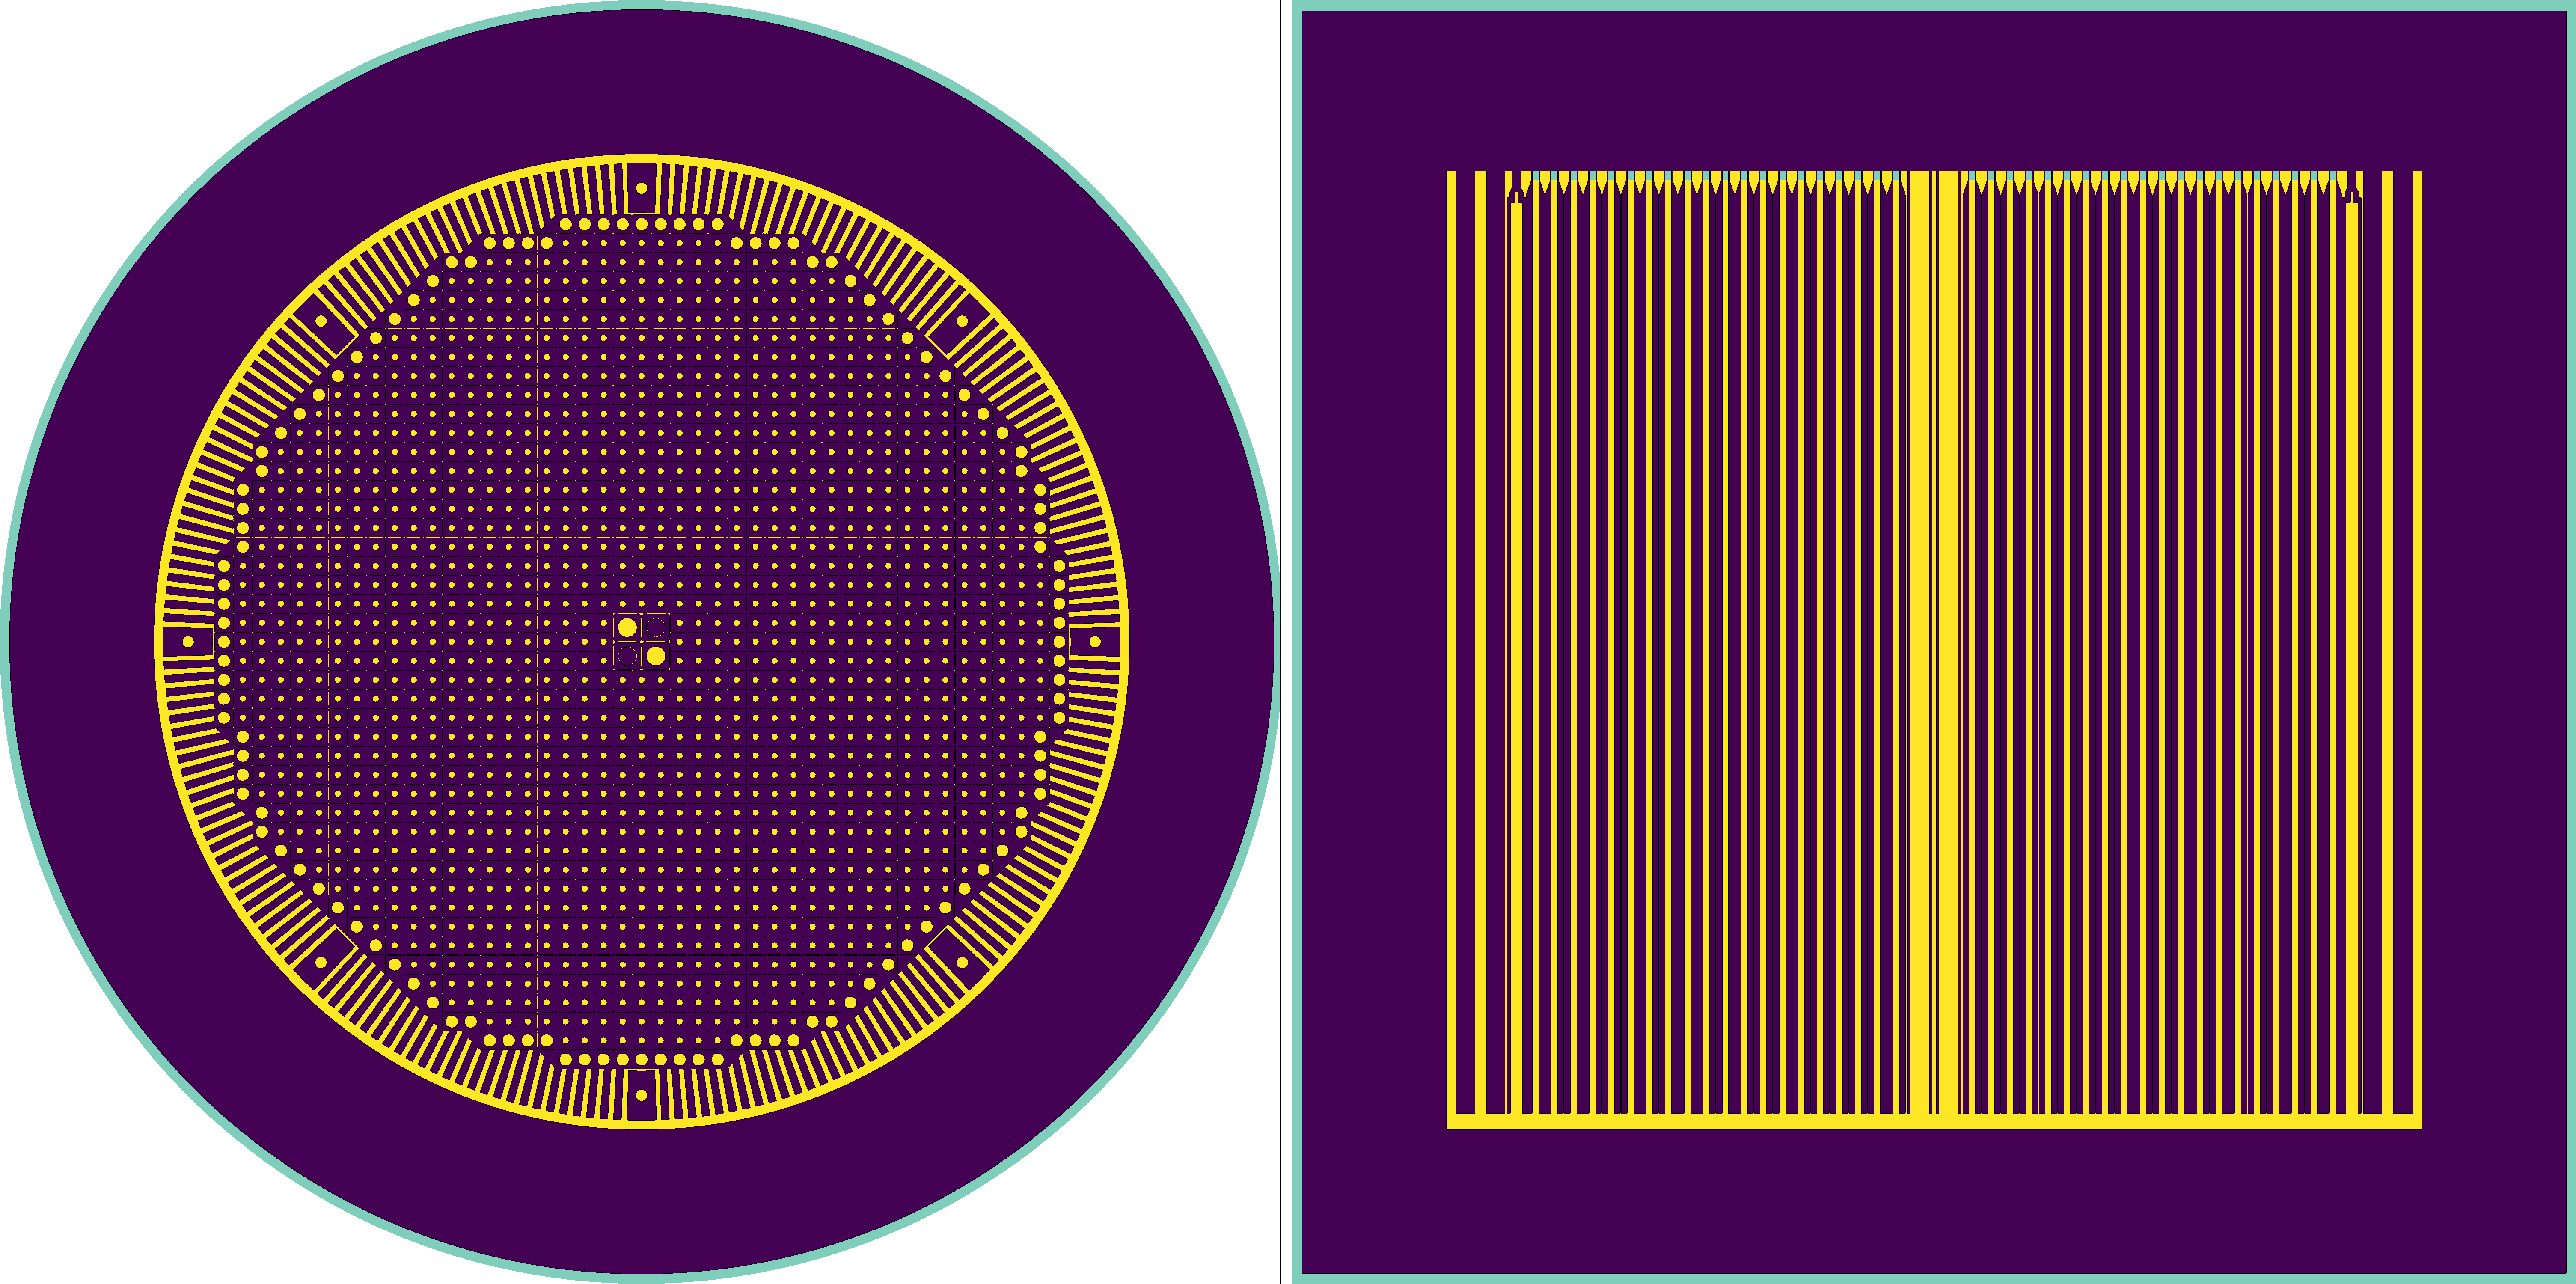
\includegraphics[width=\textwidth]{view_serpent.png}
  \caption{Plan and elevation views of SERPENT 2 \gls{MSBR} model developed in 
  this work.}
  \label{fig:serpent_plan_view}
\end{figure}

Moreover, it was decided to remove and install the core graphite as an assembly 
rather than by individual blocks, because it is relatively easier for 
maintenance personnel and has lower probability of radioactive elements escape 
due to used blocks damage during removal. In addition, handling the core as an 
assembly also allows the replacement core to be carefully preassembled and 
tested under factory conditions.

There are eight symmetric graphite slabs with a width of 15.24 cm in zone II, 
one of which is illustrated in Figure~\ref{fig:serpent_zoneII}. The holes in 
the centers are for the core lifting rods used during the core replacement 
operations. These holes also allow a portion of the fuel salt to flow to the 
top of the vessel for cooling the top head and axial reflector. 
Figure~\ref{fig:serpent_zoneII} also demonstrates the 5.08-cm-wide annular 
space between the removable core graphite in zone II-B and the permanently 
mounted reflector graphite. This annulus consists entirely of fuel salt, 
provides space for moving the core assembly, helps compensate the elliptical 
dimensions of the reactor vessel, and serves to reduce the damaging flux at the 
surface of the graphite reflector blocks. In this work, all figures of the core 
were generated using the built-in SERPENT 2 plotter. All calculations presented 
in this study were performed using SERPENT 2 version 2.1.30 on Blue Waters’ XE6 
nodes. 

\begin{figure}[t!] % replace 't' with 'b' to \centering
  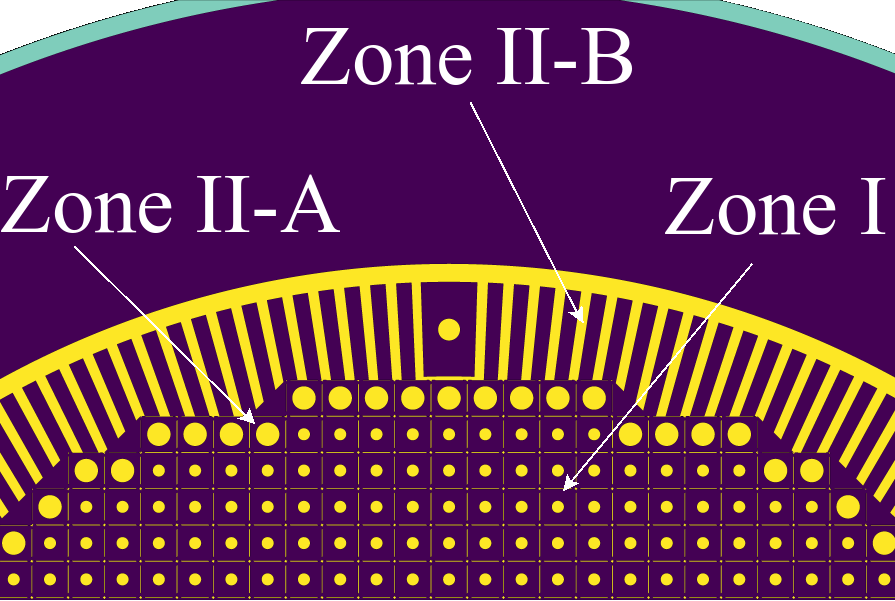
\includegraphics[width=\textwidth]{ser_zone_II.png}
  \caption{Detailed view of \gls{MSBR} zone II model.}
  \label{fig:serpent_zoneII}
\end{figure}

\subsubsection{Core zone I}
The central region of the core, called zone I, is made up of graphite elements, 
each $10.16$cm$\times$10.16cm$\times$396.24cm. Zone I has 4 channels for 
control rods: two for graphite rods which both regulate and shim during normal 
operation, and two for backup safety rods consisting of boron carbide clad to 
assure sufficient negative reactivity for emergency situations.

These graphite elements have a mostly rectangular shape with lengthwise ridges 
at each corner that leave space for salt flow elements. Various element sizes 
reduce the peak damage flux and power density in the center of the core to 
prevent local graphite damage. Zone I is well-moderated to achieve the desired 
fission power density. Figure~\ref{fig:I_element_ref} demonstrates the 
elevation and plan views of graphite elements of zone I 
\cite{robertson_conceptual_1971} and their SERPENT model 
\cite{rykhlevskii_full-core_2017}.
\begin{figure}[ht!] % replace 't' with 'b' to \centering
  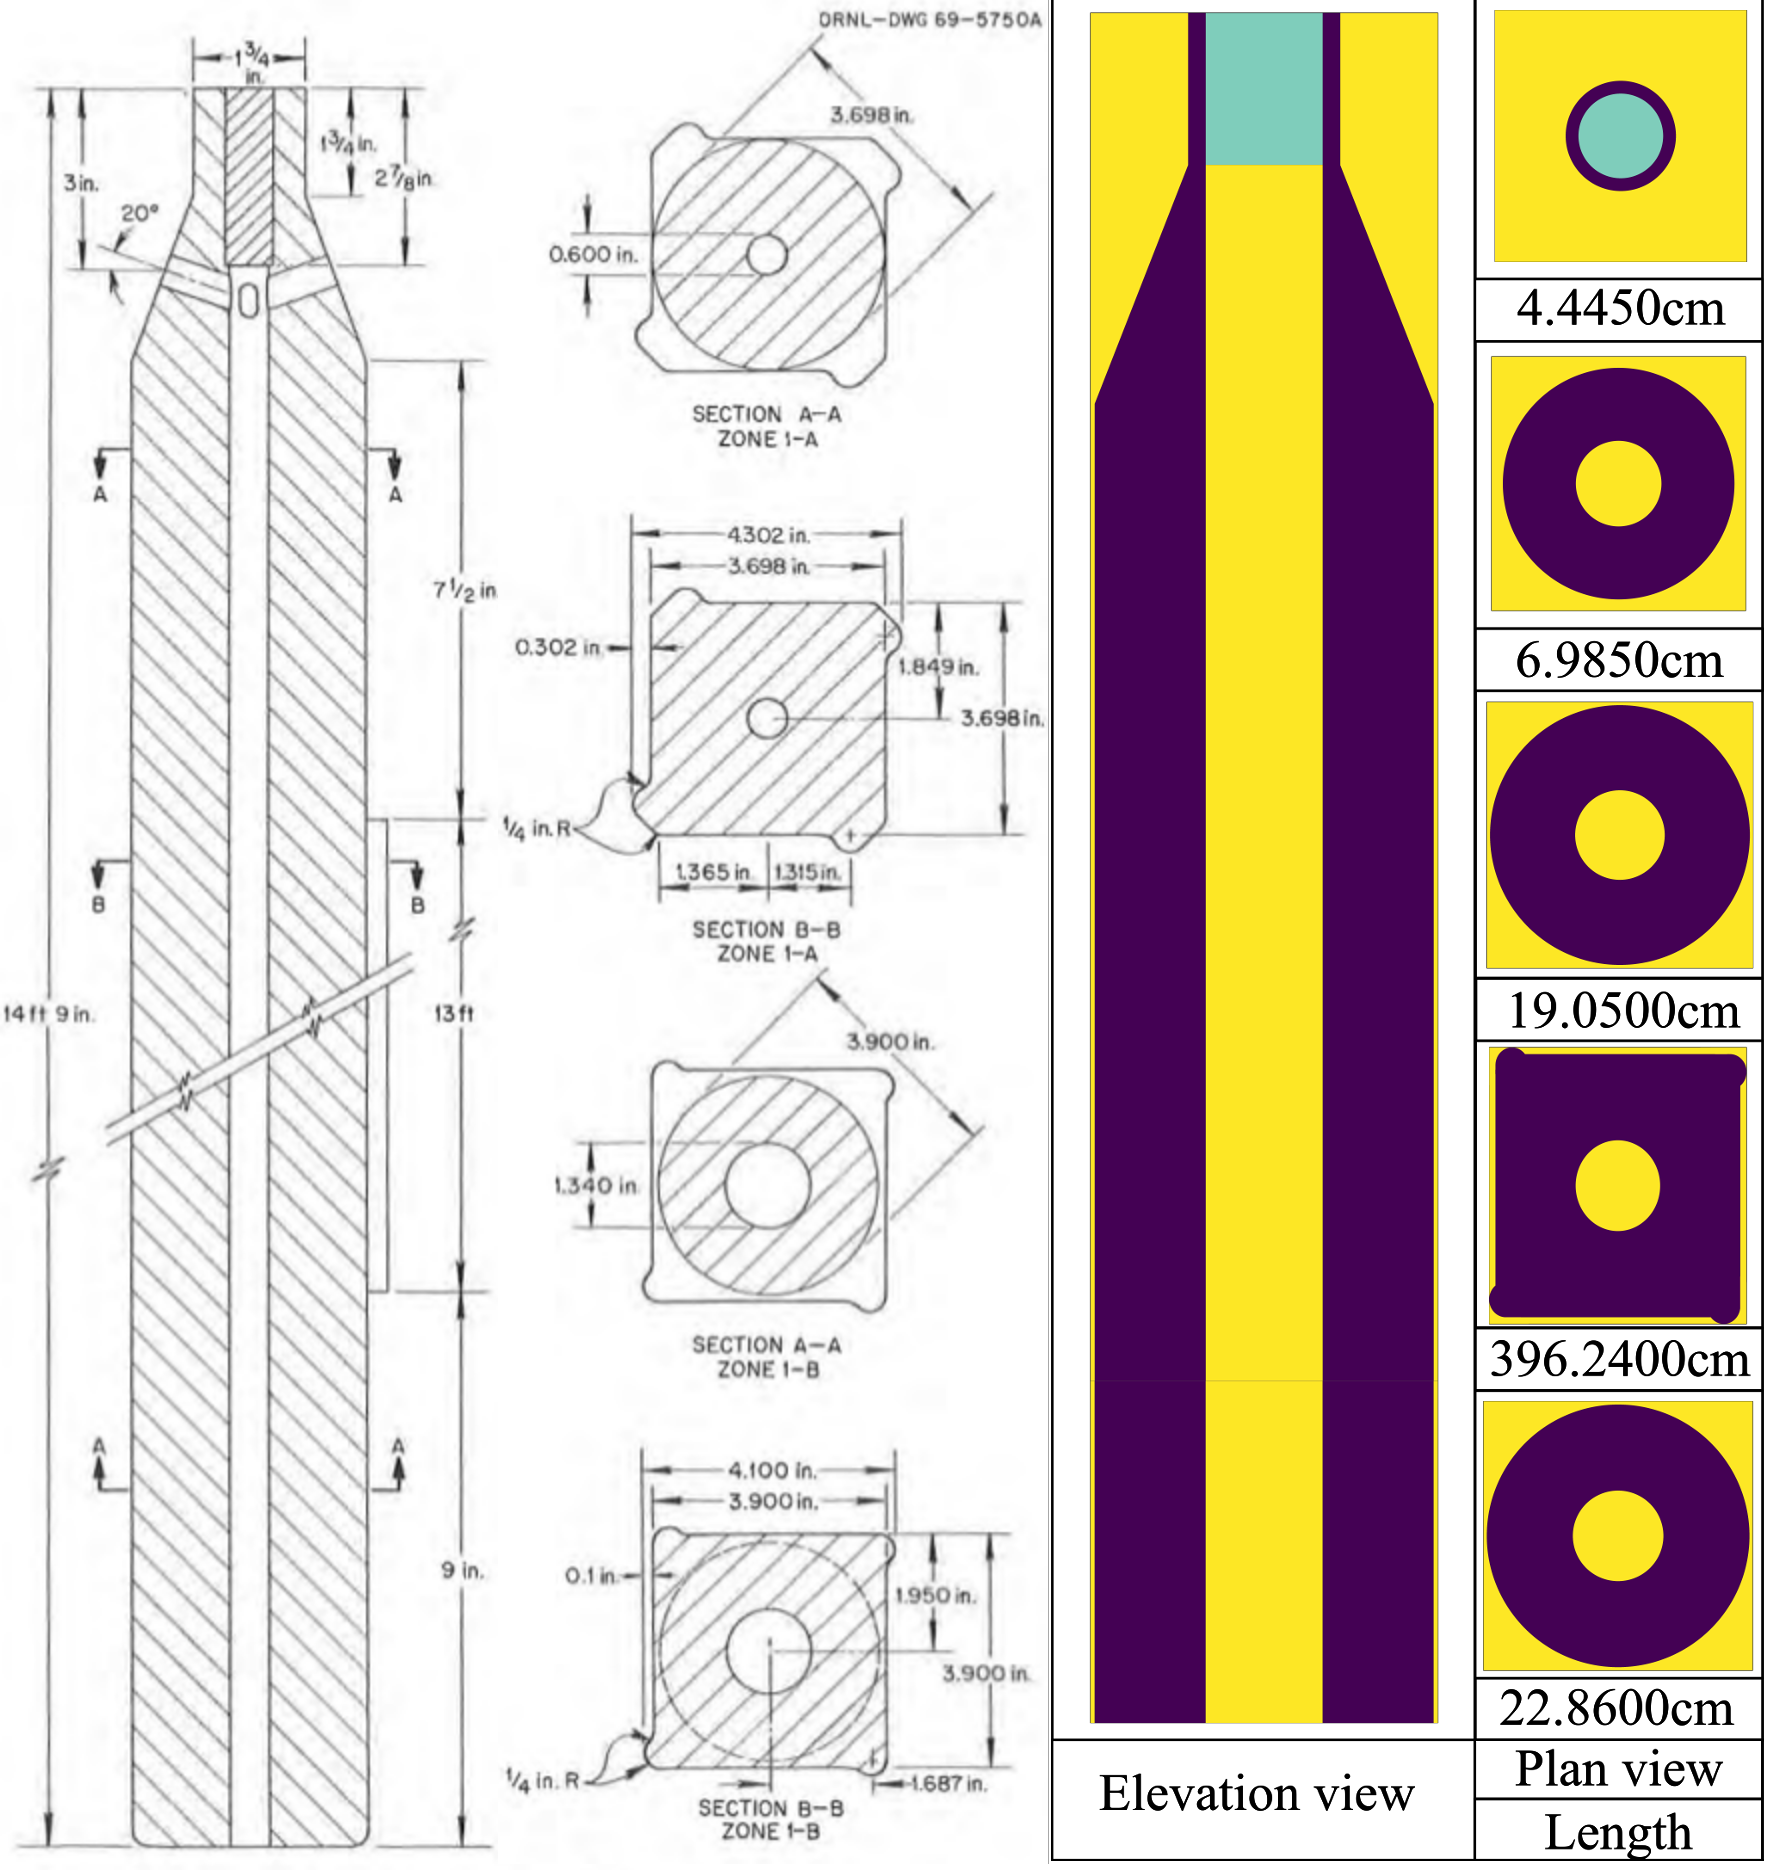
\includegraphics[width=\textwidth]{zone_I_element_ref.png}
  \caption{Graphite moderator elements for zone I 
  \cite{robertson_conceptual_1971,rykhlevskii_full-core_2017}.}
  \label{fig:I_element_ref}
\end{figure}

\subsubsection{Core zone II}
Zone II which is undermoderated, surrounds zone I. Combined with the bounding 
radial reflector, zone II serves to diminish neutron leakage. This zone is 
formed of two kinds of elements: large-diameter fuel channels (zone II-A) and 
radial graphite slats (zone II-B). 

Zone II has 37\% fuel salt by volume and each element has a fuel channel 
diameter of 6.604cm. The graphite elements for zone II-A are prismatic and have 
elliptical-shaped dowels running axially between the prisms and needed to 
isolate the fuel salt flow in zone I from that in zone II. 
Figure~\ref{fig:II_element_ref} shows shape and dimensions of these graphite 
elements and their SERPENT model. Zone II-B elements are rectangular slats 
spaced far enough apart to provide the 0.37 fuel salt volume fraction. The 
reactor zone II-B graphite 5.08cm-thick slats vary in the radial dimension 
(average width is 26.67cm) as shown in figure~\ref{fig:serpent_zoneII}. Zone II 
serves as a blanket to achieve the best performance: a high breeding ratio and 
a low fissile inventory. The neutron energy spectrum in zone II is made harder 
to enhance the rate of thorium resonance capture relative to the fission rate, 
thus limiting the neutron flux in the outer core zone and reducing the neutron 
leakage \cite{robertson_conceptual_1971}. 

The main challenge was to accurately represent zone II-B because it has 
irregular elements with sophisticated shapes. From the \gls{ORNL} report 
\cite{robertson_conceptual_1971}, the suggested design of zone II-B has 8 
irregularly-shaped graphite elements every 45$^\circ$ as well as salt channels. 
These graphite elements were simplified into right-circular cylindrical shapes  
with central channels. Figure~\ref{fig:serpent_zoneII} illustrates this core 
region in the SERPENT model. The volume of fuel salt in zone II was kept 
exactly 37\%, so that this simplification did not considerably change the core 
neutronics. This is the only simplification made to the \gls{MSBR} geometry in 
this work. 

\begin{figure}[ht!] % replace 't' with 'b' to \centering
  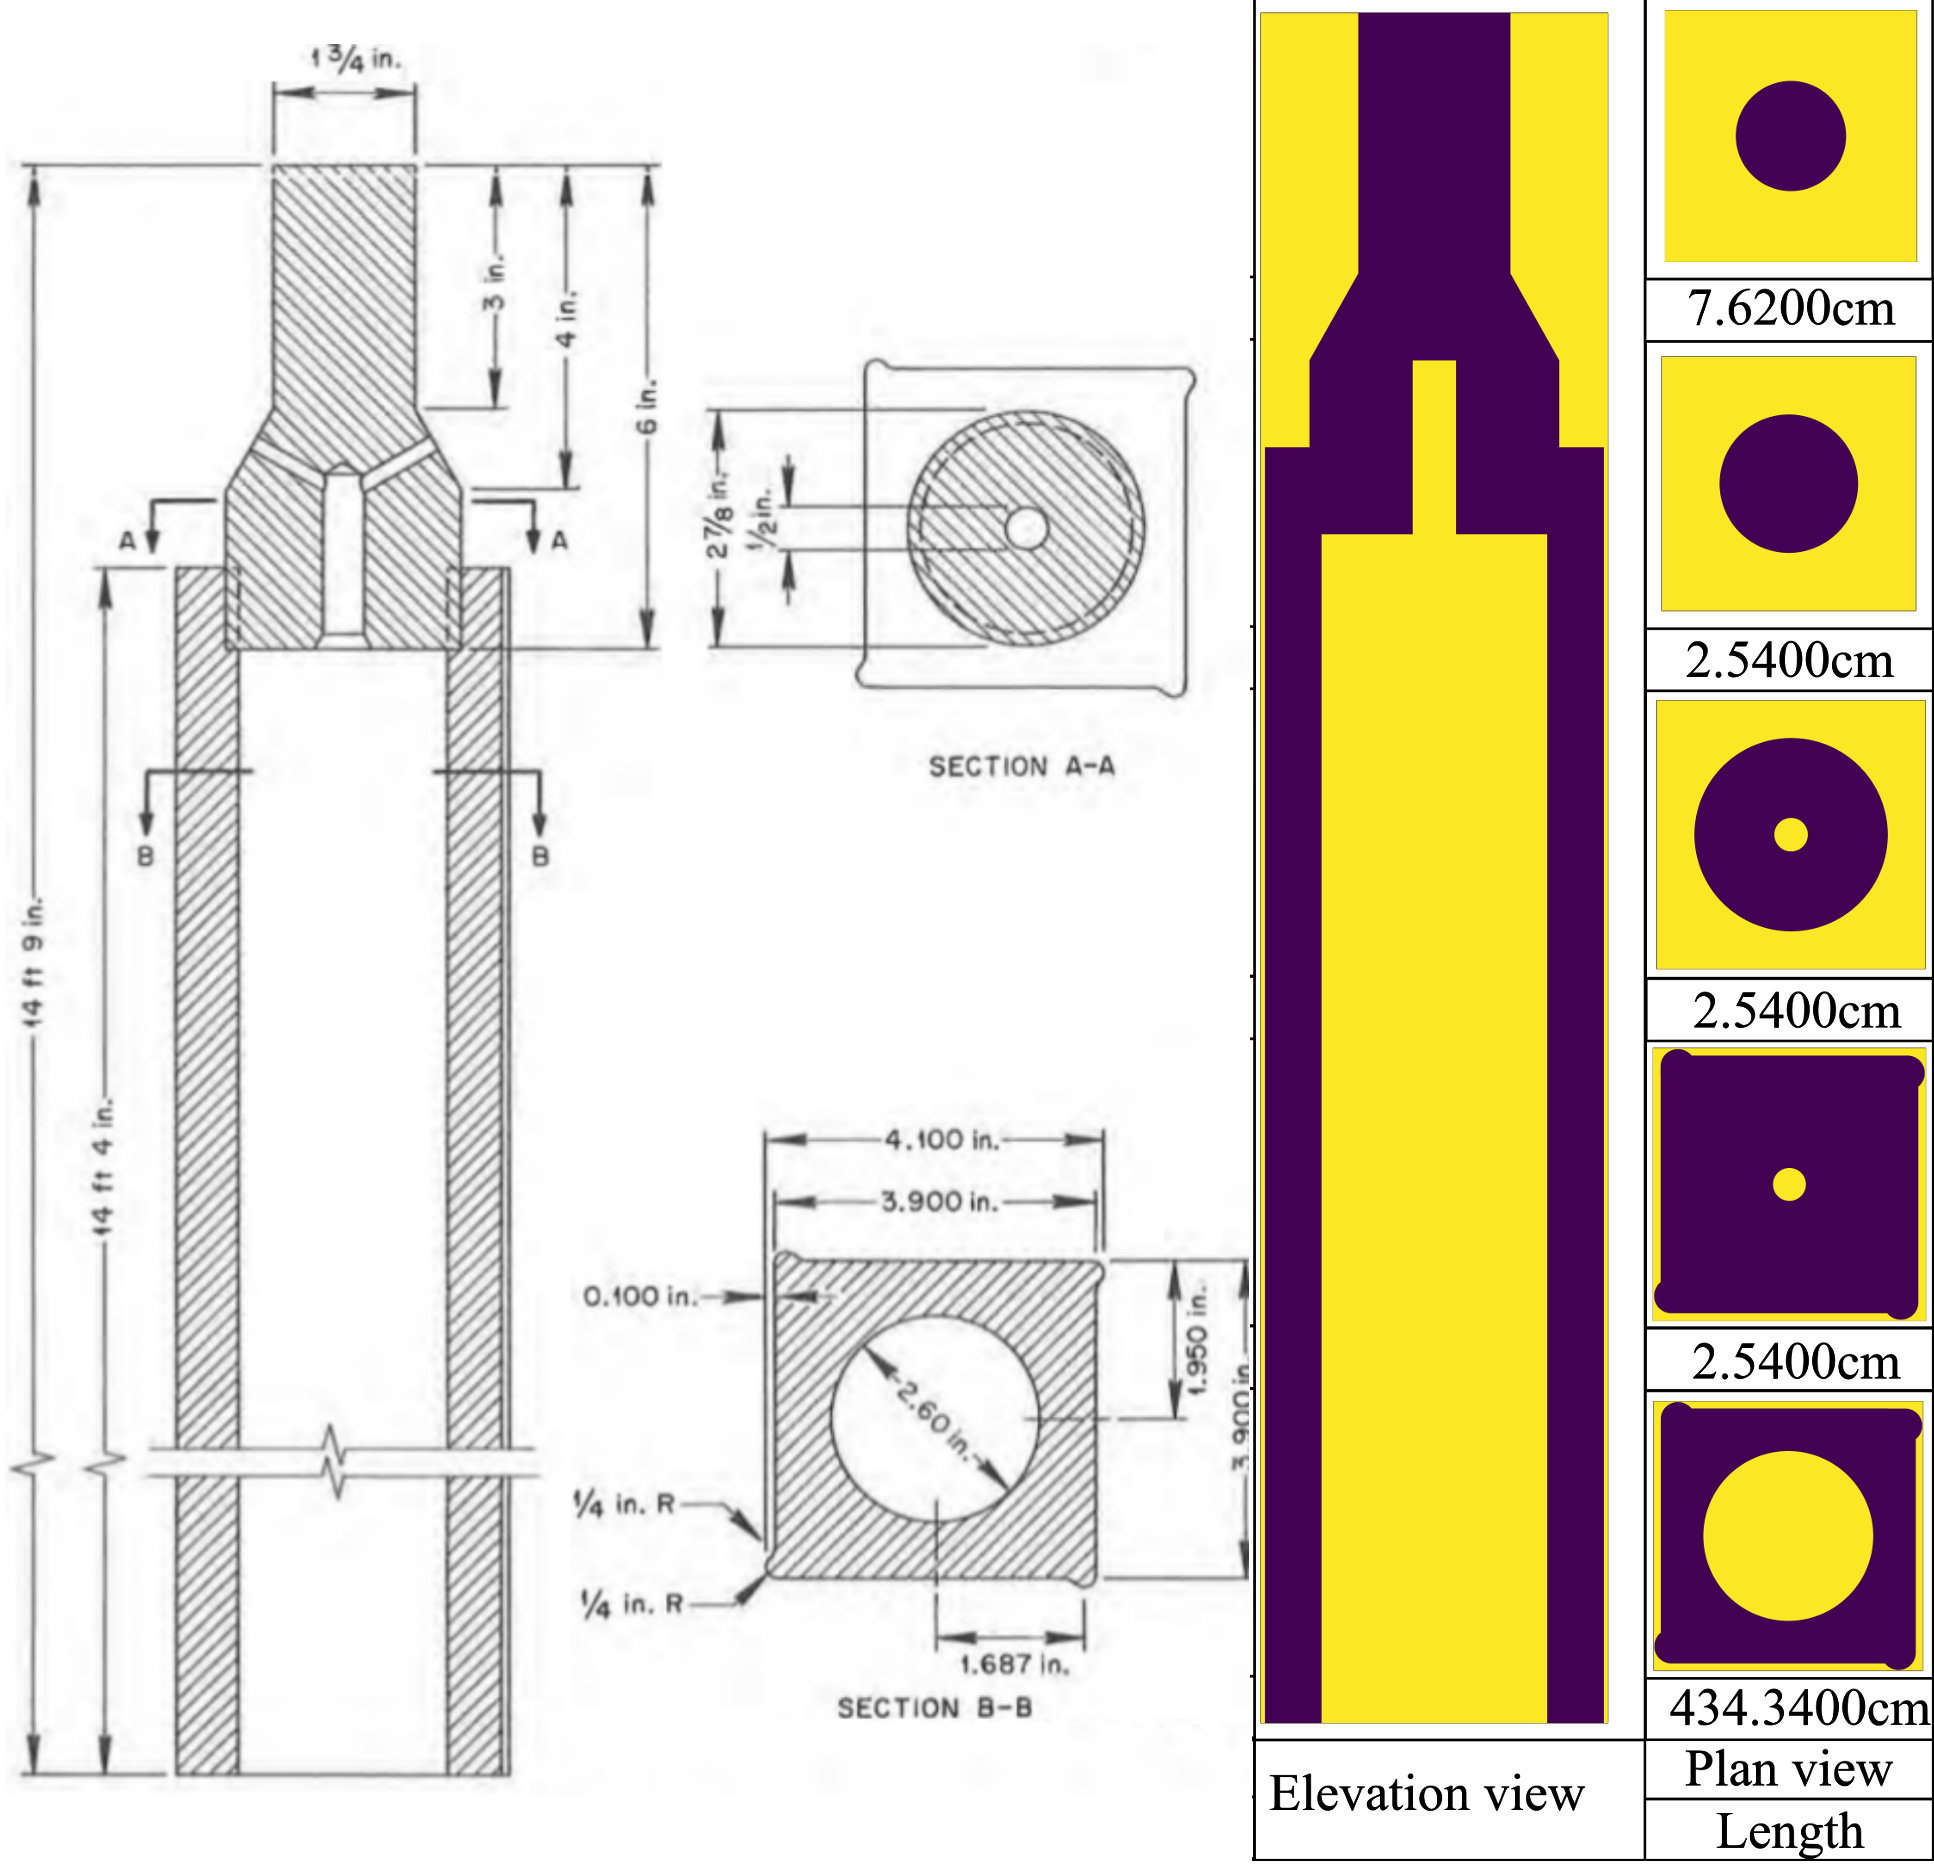
\includegraphics[width=\textwidth]{zone_II_element_ref.png}
  \caption{Graphite moderator elements for zone II-A 
  \cite{robertson_conceptual_1971,rykhlevskii_full-core_2017}.}
  \label{fig:II_element_ref}
\end{figure}

\subsubsection{Material composition and normalization parameters}
The fuel salt, the reactor graphite, and the modified Hastelloy-N\footnote{ 
Hastelloy-N is very common in reactors now but have been studied and developed 
at \gls{ORNL} in a program that started in 1950s.} are materials unique of the 
\gls{MSBR} and were created at \gls{ORNL}. The initial fuel salt used the same 
density (3.35 g/cm$^3$) and composition LiF-BeF$_2$-ThF$_4$-$^{233}$UF$_4$ 
(71.75-16-12-0.25 mole \%) as the \gls{MSBR} design 
\cite{robertson_conceptual_1971}. The lithium in the molten salt fuel is fully 
enriched in $^{7}$Li because $^{6}$Li is a very strong neutron poison and 
becomes tritium upon neutron capture. 

For cross section generation, JEFF-3.1.2 neutron library was employed 
\cite{oecd/nea_data_bank_jeff-3.1.2_2014}. The specific temperature was fixed 
for each material to correctly model the Doppler-broadening of resonance peaks 
when SERPENT generates the problem-dependent nuclear data library. The isotopic 
composition of each material at the initial state was described in detail in 
the MSBR conceptual design study \cite{robertson_conceptual_1971} and has been 
applied to SERPENT model without any modification. Table~\ref{tab:msbr_tab} is 
a summary of the major \gls{MSBR} parameters used by this model 
\cite{robertson_conceptual_1971}. 

%%%%%%%%%%%%%%%%%%%%%%%%%%%%%%%%%%%%%%%%
\begin{table}[h!]
        %\centering
        \caption{Summary of principal data for MSBR 
        \cite{robertson_conceptual_1971}.}
        \begin{tabularx}{\textwidth}{ s  s}
        \hline
                Thermal capacity of reactor           		& 2250 MW(t)
                \\ Net electrical output                 		& 1000 
        MW(e) \\  Net thermal efficiency        				
        & 44.4\%
                \\  Salt volume fraction in central zone I		& 0.13
                \\ Salt volume fraction in outer zone II       & 0.37
                \\ Fuel salt inventory (Zone I)                & 8.2 m$^3$	
        \\ Fuel salt inventory (Zone II)               & 10.8 m$^3$	\\ Fuel 
        salt inventory (annulus)               & 3.8 m$^3$	\\  Total fuel 
        salt inventory                   & 48.7 m$^3$	\\ Fissile mass in fuel 
        salt                   & 1303.7 kg	\\ Fuel salt components                  
                               & LiF-BeF$_2$-ThF$_4$-$^{233}$UF$_4$	\\  
        Fuel salt composition                 & 71.75-16-12-0.25 mole\%
                \\
                Fuel salt density                    & 3.35 g/cm$^3$
                \\ \hline
        \end{tabularx}
        \label{tab:msbr_tab}
\end{table}
%%%%%%%%%%%%%%%%%%%%%%%%%%%%%%%%%%%%%%%%%%%%%%%%

\subsection{Online reprocessing method}
Removing specific chemical elements from a molten salt is a complicated task 
that requires intelligent design (e.g., chemical separations equipment design, 
fuel salt flows to equipment) and has a considerable economic cost. All 
liquid-fueled \gls{MSR} designs involve varying levels of online fuel 
processing. Minimally, volatile gaseous fission products (e.g. Kr, Xe) escape 
from the fuel salt during routine reactor operation and must be captured. 
Additional systems might be used to enhance removal of those elements. Most 
designs also call for the removal of noble and rare earth metals from the core 
since these metals act as neutron poisons. Some designs suggest a more complex 
list of elements to process (figure ~\ref{fig:periodic_tab}), including the 
temporary removal of protactinium from the salt or other regulation of the 
actinide inventory in the fuel salt \cite{ahmad_neutronics_2015}.

\begin{figure}[htp!] % replace 't' with 'b' to \centering
  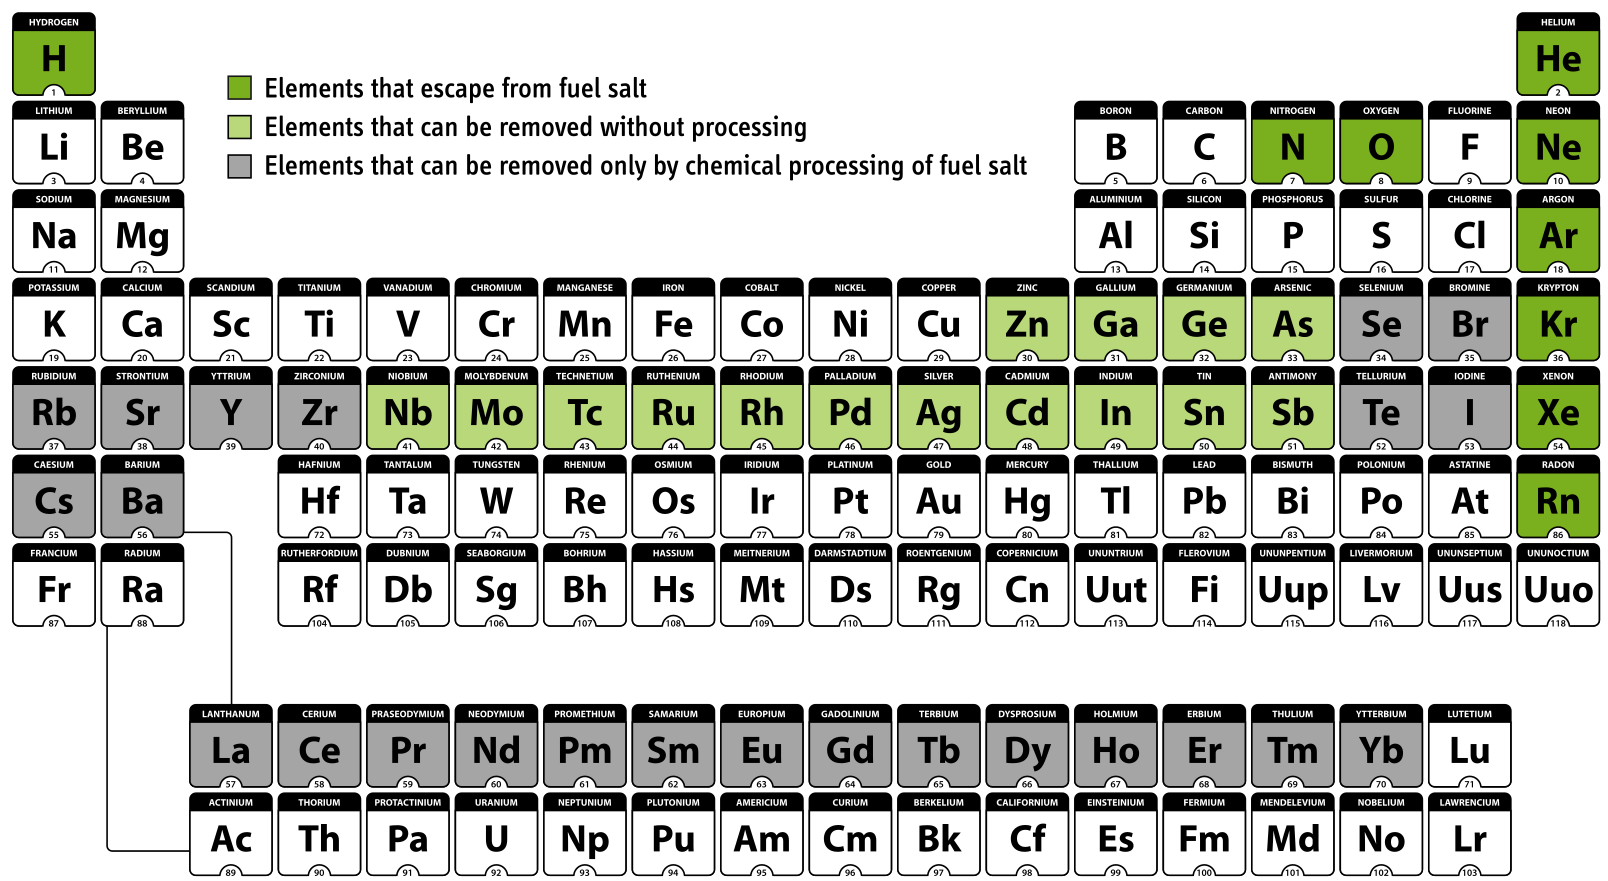
\includegraphics[width=\textwidth]{periodic_map.png}
  \caption{Processing options for \gls{MSR} fuels 
  \cite{ahmad_neutronics_2015}.}
  \label{fig:periodic_tab}
\end{figure}

\subsubsection{Fuel material flows}
The $^{232}$Th in the fuel absorbs thermal neutrons and produces $^{233}$Pa 
which then decays into the fissile $^{233}$U. Furthermore, the \gls{MSBR} 
design requires online reprocessing to remove all poisons (e.g. $^{135}$Xe), 
noble metals, and gases (e.g. $^{75}$Se, $^{85}$Kr) every 20 seconds. 
Protactinium presents a challenge, since it has a large absorption cross 
section in the thermal energy spectrum. Accordingly, $^{233}$Pa is continuously 
removed from the fuel salt into a protactinium decay tank to allow $^{233}$Pa 
to decay to $^{233}$U without poisoning the reactor. The reactor reprocessing 
system is designed to separate $^{233}$Pa from the molten-salt fuel over 3 
days, hold it while $^{233}$Pa decays into $^{233}$U, and return it back to the 
primary loop. This feature allows the reactor to avoid neutron losses to 
protactinium, keeps fission products to a very low level, and increases the 
efficiency of $^{233}$U breeding. Table~\ref{tab:reprocessing_list} summarizes 
full list of nuclides and the cycle times used for modeling salt treatment and 
separations \cite{robertson_conceptual_1971}. 

%%%%%%%%%%%%%%%%%%%%%%%%%%%%%%%%%%%%%%%%
\begin{table}[ht!]
        \centering
        \caption{The effective cycle times for protactinium and fission 
        products removal (reproduced from \cite{robertson_conceptual_1971}).}
        \begin{tabularx}{\textwidth}{ x | s | x }
        \hline Processing group & \qquad\qquad\qquad Nuclides & Cycle time (at 
                full power) \\ \hline Rare earths & Y, La, Ce, Pr, Nd, Pm, Sm, 
                Gd & 50 days \\ \qquad & Eu & 500 days \\ Noble metals & Se, 
                Nb, Mo, Tc, Ru, Rh, Pd, Ag, Sb, Te & 20 sec \\
        Seminoble metals & Zr, Cd, In, Sn & 200 days \\
        Gases & Kr, Xe & 20 sec \\ Volatile fluorides & Br, I & 60 days \\
        Discard & Rb, Sr, Cs, Ba & 3435 days \\ Salt discard & Th, Li, Be, F & 
                3435 days \\ Protactinium & $^{233}$Pa & 3 days \\ Higher 
                nuclides & $^{237}$Np, $^{242}$Pu & 16 years \\  \hline
        \end{tabularx}
        %\footnotetext{Chemical processing plant and gas separation system 
        %removing chemical elements (not isotopes) only. Isotopes instead of 
        %elements listed because other isotopes are short-lived and might be 
        %ignored.}
        \label{tab:reprocessing_list}
\end{table}
Th removal rates vary among nuclides in this reactor concept which dictate the 
necessary resolution of depletion calculations. If the depletion time intervals 
are very short, an enormous number of depletion steps are required to obtain 
the equilibrium composition. On the other hand, if the depletion  calculation 
time interval is too long, the impact of short-lived fission products is not 
captured. To compromise, the time interval for depletion calculations in this 
model was selected as 3 days to correlate with the removal interval of 
$^{233}$Pa and $^{232}$Th was continuously added to maintain the initial mass 
fraction of $^{232}$Th.

\subsubsection{The SaltProc modeling and simulation code}
The SaltProc tool \cite{andrei_rykhlevskii_arfc/saltproc:_2018} is designed to 
expand SERPENT 2
 depletion capabilities for modeling liquid-fueled \gls{MSR} for continuous 
 reprocessing.
The Python package uses HDF5 \cite{the_hdf_group_hierarchical_1997} to store 
data, and the Nuclear Engineering Toolkit PyNE \cite{scopatz_pyne:_2012}
for SEPRENT output file parsing and nuclide naming. It is an open-source tool 
that uses a semi-continuous approach to simulate continuous feeds and removals 
in the \gls{MSR}. 

The tool structure and capabilities of SaltProc are similar to ChemTriton tool 
for SCALE
developed in \gls{ORNL} \cite{powers_new_2013}. SaltProc is coupled with Monte 
Carlo SERPENT 2
software which allows to simulate online reprocessing for irregular full-core 
geometry with high level of fidelity.  The primary function of SaltProc is to 
manage material streams while
SERPENT 2 performs most of the computationally heavy work, namely neutron 
transport and depletion
calculations. Saltproc is defined as a python class, where each material stream 
is defined as a isotopic atomic density
vector variable. This allows tracking of time-sensitive material streams such 
as the
$^{233}$Pa tank in the \gls{MSBR}. The user can define the reprocessing 
parameters, such as the reprocessing interval and removal efficiency.  In 
addition, SaltProc provides a set of functions for each stream: read and write 
isotopic data in/from database, separate out specific isotopes from stream with 
defined efficiency, feed in specific isotopes to stream, and maintain constant 
number density of specific nuclide in the core. These attributes and functions 
are crucial to simulate the operation of a complex, multi-zone, multi-fluid 
\gls{MSR} and are universal for myriad reactor systems.

Saltproc is currently in active development in Github (https://github.com/ 
arfc/saltproc), and has unit tests and Travis continuous integration for 
sustainable development. There is also documentation
generated through Sphinx document generator for ease of use. We plan to 
implement
user-defined reprocessing scheme definition, two-region \gls{MSR} modeling 
capabilities,
and decay modeling in future releases.

Figure~\ref{fig:saltproc_flow} illustrates the  online reprocessing simulation 
algorithm the coupled SaltProc and SERPENT 2. To perform a depletion step,
SaltProc reads an external SERPENT 2 template file which is defined by the 
user. This file contains input cards with parameters such as geometry,
moderator and construction materials isotopic composition, neutron population, 
criticality cycles, total heating power, and boundary conditions.
After the depletion calculation, SaltProc reads the depleted fuel composition 
file (\texttt{
.bumat1}) and stores the depleted
composition isotopic vector in an HDF5 database. SaltProc only stores and edits 
the isotopic composition of the fuel stream,
which makes SaltProc a flexible tool to model any geometry: an infinite medium, 
a unit cell, a multi-zone simplified assembly, or a full core.
This flexibiliity allows the user to perform simulations of varying fidelity 
and computational intensity.
\begin{figure}[ht!] % replace 't' with 'b' to \centering
  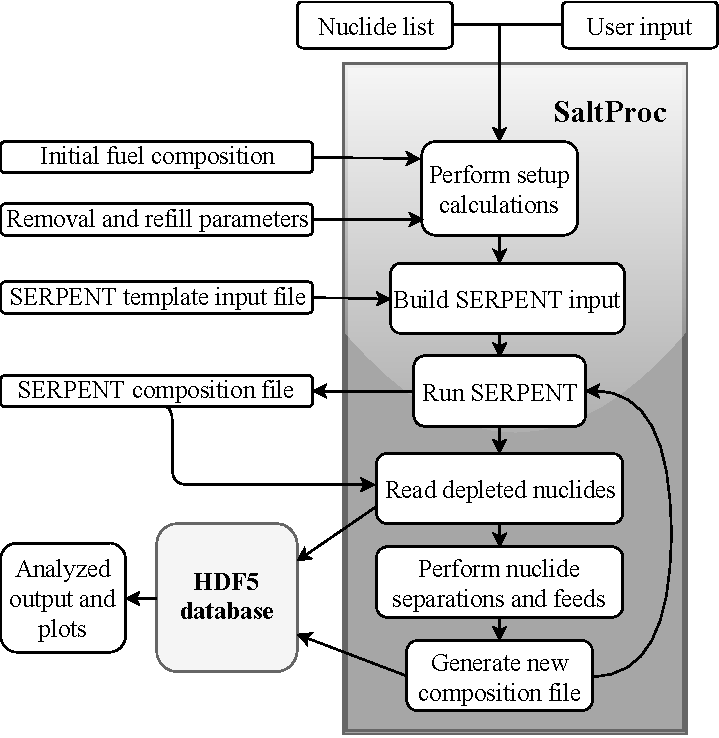
\includegraphics[width=0.75\textwidth]{saltproc_flowchart.pdf}
  \caption{Flow chart for the Saltproc python-based tools.}
  \label{fig:saltproc_flow}
\end{figure}
SaltProc can manage as many material streams as desired. It also may work with 
multiple depletion materials. At the end of a each depletion step, SaltProc 
reads the depleted compositions and tracks each material stream individually. 
Following this, it applies chemical separation functions to fuel stream 
vectors. These vectors then form a matrix (isotopics x timesteps) which 
SaltProc stores in an HDF5 database and prints into the SERPENT 2 composition 
file for the next depletion calculation.

Saltproc datasets are timseries, meaning that every value is recorded every 
timestep. The datasets SaltProc produces are listed below,
where the values inside the parenthesis are the dataset sizes:

\begin{itemize}
    \item \texttt{core adensity before reproc} (number of isotopes x timesteps)
    \item \texttt{core adensity after reproc} (number of isotopes x timesteps)
    \item \texttt{Keff\_BOC} (1 x timesteps)
    \item \texttt{Keff\_EOC} (1 x timesteps)
    \item \texttt{Th tank adensity} (number of isotopes x timesteps)
    \item \texttt{iso codes} (number of isotopes x 1)
\end{itemize}

Liquid-fueled \gls{MSBR} design in this work focuses on the state of the core 
at an equilibrium condition, after fission products have built up in the fuel 
salt during years if operation. Isotopic composition of the fuel salt continues 
change slightly even after decades of operation, but the dominant nuclides that 
have significant impact to the neutronic behavior tend to reach an equilibrium 
concentration (e.g., vary less than 1\% over several years). In contrast, from 
the startup of an \gls{MSBR} until the equilibrium condition, the fuel salt 
composition undergoes significant changes (e.g., changes in fission products, 
minor actinides, and fissile materials number density). During this period, the 
material feeds and removals should be optimized for the fastest \gls{MSBR} 
transition to an equilibrium state. A faster transition simplifies the reactor 
operation because, at equilibrium, the fissile and fertile feed rates, fission 
product removal rates, and corresponding core safety parameters are constant in 
time.

In addition, SaltProc is able to define time-dependent material feed and 
removal rates to investigate the their impacts. These rates need not be 
constant in SaltProc. They can be defined as piecewise functions or set to 
respond conditions in the core. For instance, SaltProc might increase the 
fissile material feeding rate if the effective multiplication factor, 
$k_{eff}$, falls below a specific limit (e.g., 1.002).
These capabilities allow SaltProc to analyze fuel cycle of a generic 
liquid-fueled \gls{MSR}. In summary, the development approach of SaltProc 
focused on producing a generic, flexible and expandable tool to give the 
SERPENT 2 Monte Carlo code the ability to conduct advanced in-reactor fuel 
cycle analysis as well as simulate a myriad of online refueling and fuel 
reprocessing systems.
